\documentclass[10pt,a4paper,conference]{IEEEtran}

% Some very useful LaTeX packages include:
% (uncomment the ones you want to load)

% *** CITATION PACKAGES ***
%
\ifCLASSOPTIONcompsoc
  % IEEE Computer Society needs nocompress option
  % requires cite.sty v4.0 or later (November 2003)
  \usepackage[nocompress]{cite}
\else
  % normal IEEE
  \usepackage{cite}
\fi
% cite.sty was written by Donald Arseneau
% V1.6 and later of IEEEtran pre-defines the format of the cite.sty package
% \cite{} output to follow that of IEEE. Loading the cite package will
% result in citation numbers being automatically sorted and properly
% "compressed/ranged". e.g., [1], [9], [2], [7], [5], [6] without using
% cite.sty will become [1], [2], [5]--[7], [9] using cite.sty. cite.sty's
% \cite will automatically add leading space, if needed. Use cite.sty's
% noadjust option (cite.sty V3.8 and later) if you want to turn this off.
% cite.sty is already installed on most LaTeX systems. Be sure and use
% version 4.0 (2003-05-27) and later if using hyperref.sty. cite.sty does
% not currently provide for hyperlinked citations.
% The latest version can be obtained at:
% http://www.ctan.org/tex-archive/macros/latex/contrib/cite/
% The documentation is contained in the cite.sty file itself.
%
% Note that some packages require special options to format as the Computer
% Society requires. In particular, Computer Society  papers do not use
% compressed citation ranges as is done in typical IEEE papers
% (e.g., [1]-[4]). Instead, they list every citation separately in order
% (e.g., [1], [2], [3], [4]). To get the latter we need to load the cite
% package with the nocompress option which is supported by cite.sty v4.0
% and later. Note also the use of a CLASSOPTION conditional provided by
% IEEEtran.cls V1.7 and later.


% *** GRAPHICS RELATED PACKAGES ***
%
  \usepackage[pdftex]{graphicx}
  \graphicspath{{../Figures/}}
  \DeclareGraphicsExtensions{.pdf,.png}
  \usepackage{color}

% *** MATH PACKAGES ***
%
\usepackage[cmex10]{amsmath}
% A popular package from the American Mathematical Society that provides
% many useful and powerful commands for dealing with mathematics. If using
% it, be sure to load this package with the cmex10 option to ensure that
% only type 1 fonts will utilized at all point sizes. Without this option,
% it is possible that some math symbols, particularly those within
% footnotes, will be rendered in bitmap form which will result in a
% document that can not be IEEE Xplore compliant!
%
% Also, note that the amsmath package sets \interdisplaylinepenalty to 10000
% thus preventing page breaks from occurring within multiline equations. Use:
%\interdisplaylinepenalty=2500
% after loading amsmath to restore such page breaks as IEEEtran.cls normally
% does. amsmath.sty is already installed on most LaTeX systems. The latest
% version and documentation can be obtained at:
% http://www.ctan.org/tex-archive/macros/latex/required/amslatex/math/

%\usepackage{amssymb}%............................ AMS Symbol fonts



% *** SPECIALIZED LIST PACKAGES ***
%
%\usepackage{algorithmic}
% algorithmic.sty was written by Peter Williams and Rogerio Brito.
% This package provides an algorithmic environment for describing algorithms.
% You can use the algorithmic environment in-text or within a figure
% environment to provide for a floating algorithm. Do NOT use the algorithm
% floating environment provided by algorithm.sty (by the same authors) or
% algorithm2e.sty (by Christophe Fiorio) as IEEE does not use dedicated
% algorithm float types and packages that provide these will not provide
% correct IEEE style captions. The latest version and documentation of
% algorithmic.sty can be obtained at:
% http://www.ctan.org/tex-archive/macros/latex/contrib/algorithms/
% There is also a support site at:
% http://algorithms.berlios.de/index.html
% Also of interest may be the (relatively newer and more customizable)
% algorithmicx.sty package by Szasz Janos:
% http://www.ctan.org/tex-archive/macros/latex/contrib/algorithmicx/

% *** ALIGNMENT PACKAGES ***
%
\usepackage{array}
% Frank Mittelbach's and David Carlisle's array.sty patches and improves
% the standard LaTeX2e array and tabular environments to provide better
% appearance and additional user controls. As the default LaTeX2e table
% generation code is lacking to the point of almost being broken with
% respect to the quality of the end results, all users are strongly
% advised to use an enhanced (at the very least that provided by array.sty)
% set of table tools. array.sty is already installed on most systems. The
% latest version and documentation can be obtained at:
% http://www.ctan.org/tex-archive/macros/latex/required/tools/


\usepackage{mdwmath}
\usepackage{mdwtab}
% Also highly recommended is Mark Wooding's extremely powerful MDW tools,
% especially mdwmath.sty and mdwtab.sty which are used to format equations
% and tables, respectively. The MDWtools set is already installed on most
% LaTeX systems. The lastest version and documentation is available at:
% http://www.ctan.org/tex-archive/macros/latex/contrib/mdwtools/

% IEEEtran contains the IEEEeqnarray family of commands that can be used to
% generate multiline equations as well as matrices, tables, etc., of high
% quality.

% *** SUBFIGURE PACKAGES ***
\ifCLASSOPTIONcompsoc
  \usepackage[caption=false,font=normalsize,labelfont=sf,textfont=sf]{subfig}
\else
  \usepackage[caption=false,font=footnotesize]{subfig}
\fi

%Setting captions to centered (Not IEEE journal standard)
%\makeatletter
%\long\def\@makecaption#1#2{\ifx\@captype\@IEEEtablestring%
%\footnotesize\begin{center}{\normalfont\footnotesize #1}\\
%{\normalfont\footnotesize\scshape #2}\end{center}%
%\@IEEEtablecaptionsepspace
%\else
%\@IEEEfigurecaptionsepspace
%\setbox\@tempboxa\hbox{\normalfont\footnotesize {#1.}~~ #2}%
%\ifdim \wd\@tempboxa >\hsize%
%\setbox\@tempboxa\hbox{\normalfont\footnotesize {#1.}~~ }%
%\parbox[t]{\hsize}{\normalfont\footnotesize \noindent\unhbox\@tempboxa#2}%
%\else
%\hbox to\hsize{\normalfont\footnotesize\hfil\box\@tempboxa\hfil}\fi\fi}
%\makeatother


% *** FLOAT PACKAGES ***
%
\usepackage{fixltx2e}
% fixltx2e, the successor to the earlier fix2col.sty, was written by
% Frank Mittelbach and David Carlisle. This package corrects a few problems
% in the LaTeX2e kernel, the most notable of which is that in current
% LaTeX2e releases, the ordering of single and double column floats is not
% guaranteed to be preserved. Thus, an unpatched LaTeX2e can allow a
% single column figure to be placed prior to an earlier double column
% figure. The latest version and documentation can be found at:
% http://www.ctan.org/tex-archive/macros/latex/base/

% *** PDF, URL AND HYPERLINK PACKAGES ***
%
\usepackage{url}

\usepackage{sistyle}
    \SIstyle{S-Africa}
    \SIunitspace{{\cdot}}
    \SIunitdot{{\cdot}}

% generate nice bookmarks and hyperrefs when exporting to pdf and dvi (screen version):
\usepackage[a4paper,plainpages=false,colorlinks,linktocpage,bookmarks=true,bookmarksopen=false]{hyperref}
% use this for printing only (no color, print version):
%\usepackage[a4paper,plainpages=false,colorlinks=false,linktocpage,bookmarks=true,bookmarksopen=false]{hyperref}

% correct bad hyphenation here
\hyphenation{op-tical net-works semi-conduc-tor}

%Add elegant support for Big-O notation
\providecommand{\OO}[1]{\operatorname{O}\left(#1\right)}

\begin{document}

%
% paper title
\title{Pithos: A Hybrid Multi-Tiered State Persistency Architecture for Peer-to-Peer Massively Multiuser Virtual Environments}

%\author{\IEEEauthorblockN{John S. Gilmore and Herman A. Engelbrecht\\}
%\IEEEauthorblockA{MIH Media Lab\\
%Electronic Engineering Department\\
%Stellenbosch University\\
%Stellenbosch, South Africa\\
%mail: jgilmore@ml.sun.ac.za and hebrecht@sun.ac.za}}

\maketitle

\begin{abstract}
%\boldmath
The abstract goes here

\end{abstract}


\section{Introduction}
\label{introduction}

%
% Admittedly, this is a hack and may well be fragile, but seems to do the
% trick for me. Note the need to keep any \label that may be used right
% after \section in the above as the hack puts \section within a raised box.

% The very first letter is a 2 line initial drop letter followed
% by the rest of the first word in caps (small caps for compsoc).
%
% form to use if the first word consists of a single letter:
% \IEEEPARstart{A}{demo} file is ....
%
% form to use if you need the single drop letter followed by
% normal text (unknown if ever used by IEEE):
% \IEEEPARstart{A}{}demo file is ....
%
% Some journals put the first two words in caps:
% \IEEEPARstart{T}{his demo} file is ....
%

%P2P MMVE Background
\IEEEPARstart{P}{eer-to-Peer (P2P)} Massively Multiuser Virtual Environments (MMVEs) have received significant attention from the research community,
since the first publication on the subject by Knutssonn et al. in 2004 \cite{knutsson_p2p_first}. P2P MMVEs promise to solve many issues prevalent in
today's Client/Server (C/S) based MMVEs. Some key issues have to be solved before P2P MMVEs can be implemented commercially. Over the past few years,
researchers have been addressing these challenges.

%Key challenges and focus
A recent article has identified six key challenges of P2P systems: Interest Management, Game Event Dissemination, Non-player Character (NPC) Host
Allocation, Game State Persistency, Cheating Mitigation and Incentive Mechanisms \cite{Fan_deisgn_issues_p2p}. Most of the challenges mentioned have
received significant attention from the research community, except for state persistency.

The focus of this paper is exclusively on one of the key challenges present in P2P MMVEs, namely: state persistency. The implementation of state
persistency in P2P MMVEs allows for the storage of game data. The fact that game data must now be distributed amongst various peers in the network
creates challenges not usually present in classic C/S MMVEs.

%Current techniques not perfect
This paper shows that none of the approaches to state persistency has thus far been sufficient to meet the storage requirements of MMVEs of today.
All storage models are evaluated according to the identified requirements of scalability, fairness, reliability, responsiveness and security.

%Propose multi-tiered model
Because current state persistency models do not address all the requirements of modern MMVEs, a novel hybrid multi-tiered state persistency model is
proposed that is based on grouping players in some logical way and allowing for responsive interaction between players in the same group, with lower
levels of responsiveness between groups.

%Implementation
The proposed multi-tiered model is currently being implemented in Oversim, a peer-to-peer simulation environment based in Omnet++. The model allows
for the measurement of the requirements of scalability, fairness, reliability and responsiveness. Furthermore, it allows for the comparison of the
current model with other state persistency models. Multiple P2P routing overlays have already been implemented in Oversim, which makes it possible
for the substitution of different overlays and comparing the results.

%Promising preliminary results
Initial results seem promising, with the implemented model functioning as expected. The system shows to be very responsive when storing data within a
group and as responsive as storing data in an overlay when storing data between groups.

%Summary
Section \ref{current_models} groups storage models found in the literature and describes the advantages and disadvantages of each group. The section
concludes with a comparison of the different storage models and comments on their applicability to P2P MMVEs.
%
Section \ref{proposed_model} introduces our proposed state persistency model and describes the different assumptions on which it is based.
%
Section \ref{implementation} describes the implementation details of the proposed model.
%
Section \ref{results} presents some preliminary results.
%
Section \ref{conclusion} concludes with a summary of the paper and a discussion on possible future work.

\section{Current state persistency models}
\label{current_models}

%Overview of four approaches
Four approaches have been identified by which state persistency is achieved in P2P MMVEs. These are: \emph{super peer storage}, \emph{overlay
storage}, \emph{distance-based storage} and \emph{hybrid storage}. Requirements have also been identified by which storage systems should be
measured. These are: scalability, fairness, reliability, responsiveness and security.

%Scalability
%Reliability
%Fairness
For a system to be fair, the responsibility of storage should be equally shared amongst all users. Ideally, a fair scheme should take the
heterogeneity of peers into account. This ensures that costs due to bandwidth and storage are shared amongst all users.
%Responsiveness
%Security

To clarify what type of objects are stored in these types, only the root objects, also called the authoritive objects, are considered for storage. It
is still assumed that replica objects that are used by players to render the world are locally stored and that these objects derive their states from
the respective root objects.

\begin{table*}[htbp]
\centering
\begin{tabular}{|r|c|c|c|c|}
\hline
Storage type & Reliability & Responsiveness & Security & Fairness\\
\hline
Super Peer & Medium & High & Low & Low\\
Overlay & High & Low & Medium & High\\
Hybrid & High & High & Medium & Low\\
Distance-based & Medium & High & Low & Medium\\
\hline
\end{tabular}
\caption{Differences between storage mechanisms} \label{tab_storage}
\end{table*}
%
Table \ref{tab_storage} presents a characterisation of current storage systems according to the characteristics defined. Table \ref{tab_storage} also
provides some references that act as examples of the different storage types mentioned. These example architectures will be discussed briefly in the
sections to follow.

\subsection{Super peer storage}

%Super peer storage - description
Super peer storage relies on the super peer storing all information that is in its domain \cite{knutsson_p2p_first}. A domain is usually created by
segmenting the world into regions and super peers act as regional servers to all peers in their region. Each super peer handles state persistency for
its region, hosting NPCs, objects and persistent player data. This storage method is much like a Client/Server setup, with the super peer acting as
the server for the virtual geographic region assigned to it.

The advantage of super peer storage is that it's fairly simple to implement using well known database solutions.

The disadvantages of super peer storage stem from the per-region centralised approach. It is difficult to achieve high levels of reliability, without
some migration mechanism that requires redundant super peers per region and allows for migration of data and responsibilities when a super peer
leaves the network. Because super peers are merely users in the virtual world, they can be expected to regularly join and leave the world. It is
possible to implement such mechanisms, although that would significantly complicate the implementation task. No current architectures are known to
have implemented such a mechanism so the difficulties associated with this approach have not been explored.

The main issues with super peer storage are those of fairness and security. Because a single super peer controls all data in a region and because
that super peer is merely another user, there might be a high possibility that the data can be compromised in some way. There is also a high
incentive to be able to modify data in a region by a user operating in that region. It is also difficult to secure the data, because any user should
have access to, for example, another user's position. If the super peer user can identify which data is which, he might be able to modify that data.

Fairness is another issue with super peer storage, because the super peers are expected to store all the region data and are also expected to donate
their bandwidth to service requests for data from all region peers.


\subsection{Overlay storage}

%Description
Overlay storage is classified as using any type of structured P2P overlay to store data in a distributed fashion \cite{Douglas05enablingmassively},
\cite{using_freenet_storage}, \cite{Fan_phd}, \cite{past_storage_focus}. This is a very broad definition, which basically encompasses any P2P
distributed storage currently in use. Some examples and a comparison of different distributed storage techniques can be found in
\cite{Hasan_distributed_storage_survey}. The reasoning is that any P2P distributed storage can be used to only store game files. Therefore,
distributed storage is used as a distributed database for game files.

%Advantages/Disadvantages


\subsection{Hybrid storage}

%Description
The world is divided into regions, with each region controlled by a super peer \cite{zoned_federation}, \cite{hybrid_storage1}. The complete region
state is cached at every super peer, the same as with super peer storage. There also exists a backup overlay storage architecture, to which data may
be backed up for long term, redundant and secure storage. The hybrid region-based overlay storage contains many improvements over pure overlay
storage as will be discussed in the following sections.

%Advantages/Disadvantages


\subsection{Distance-based storage}

%Description
Distance based approaches, such as the Voronoi storage approaches \cite{Buyukkaya_voronoi_state_management}, \cite{Hu_voronoi_IM} and some more
general approaches \cite{colyseus_distance_based}, \cite{solipsis}, store object data on the peer closest to the object in the virtual world. Some
distance metric is used to determine on which node an object should be stored.

individual storage \cite{individual_storage1}, \cite{cheat_proof_playout}

\begin{figure}[htbp]
 \centering
 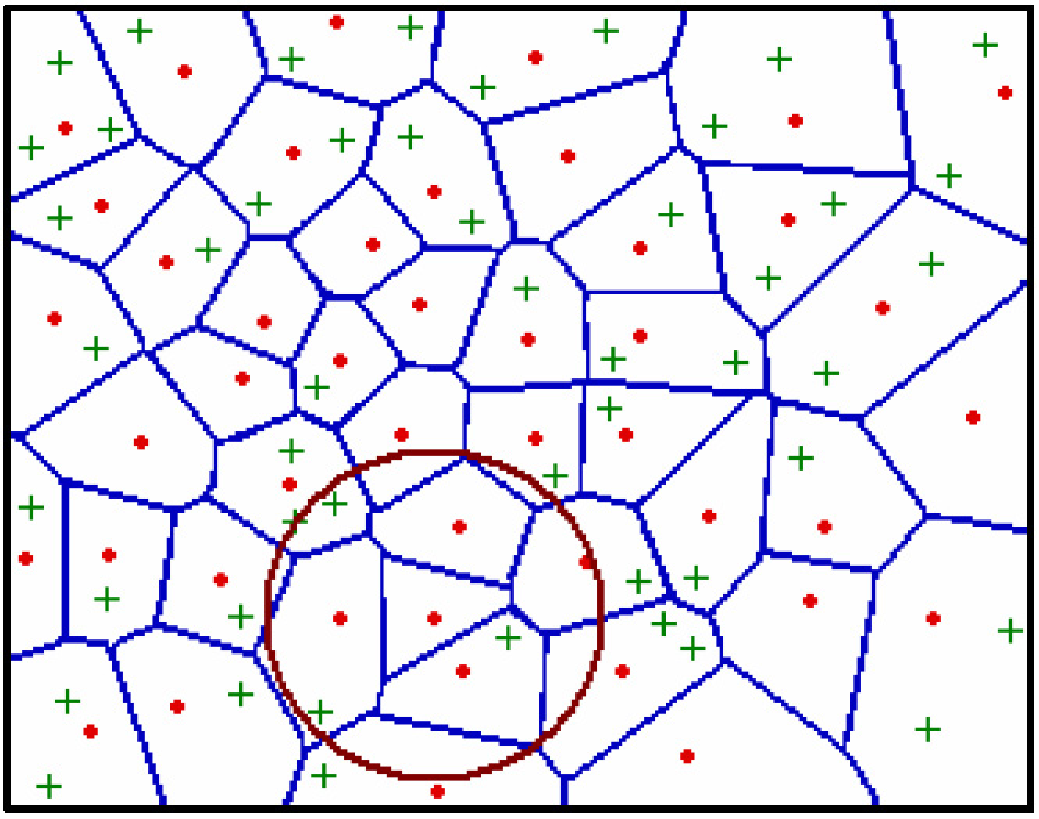
\includegraphics[width=0.7\columnwidth]{voronoi_diagram}
 \caption{Voronoi Diagram \cite{Buyukkaya_voronoi_state_management}}
 \label{fig_voronoi_diagram}
\end{figure}
%
Given a set of points, the Voronoi diagram of the set of points is the partition of the plane, which associates a region around every point in such a
way that all other points contained in the region are closer to the centre point than any other point in the set. Figure \ref{fig_voronoi_diagram}
shows a Voronoi diagram, where the lines define the region boundaries, the dots define the players, which make up the set of points for which the
diagram was calculated, the plus signs represent mutable objects and the circle represents the AoI of a central point in the set.

For the Voronoi approaches, described in more detail in Section \ref{distance_based_existing_archs}, a node controls and hosts all objects within its
Voronoi region. The reasoning is that there is a high probability that the player closest to the object is also the player using the object. Examples
of this are where a player is trading or fighting with an NPC.

%Advantages/Disadvantages

\subsection{Centralised storage}

%Description
Some P2P MMVEs use centralised storage, where all peers store data in a centralised database \cite{badumna_engine},
\cite{rooney_centralised_storage}, \cite{hybrid_p2p_cs_centralised}.

%Advantages/Disadvantages
This type of storage suffers from all the scalability and single point of failure issues present in a centralised system. Consequently, most of the
advantages of P2P MMVEs are forgone by this type of storage. When compared to the requirements mentioned in Section \ref{current_models}, centralised
storage suffers from fairness and reliability issues.

%Advantages/Disadvantages


\subsection{Summary and comparison}

From this discussion, it is evident that none of the mentioned storage types in their current forms are appropriate for data storage in MMVEs. None
of the storage types meet all the requirements as set out. Super peer storage is not fair or secure, overlay storage is not responsive, hybrid
overlay/super peer storage is not fair and distance-based storage is not secure and not yet reliable.

It should also be noted that most of these storage types are not mature. In the referenced papers, they were mentioned as a means by which
persistency might be achieved. But none of the papers presented concrete design, implementation and results on the performance of the storage types,
except for the PAST implementation, which is an overlay storage type.

This shows that not only is a storage type required that improves upon past storage types, but a concrete design and implementation is also required
that would lay bare any unforeseen issues that might arise when implementing P2P MMVEs. The following sections attempt to provide such a design and
such an implementation.

While the system is not yet complete, some promising preliminary results are also shown. These results show the improvements in terms of
responsiveness and fairness achieved.

\section{Pithos: the proposed state persistency model}
\label{proposed_model}

In this section ``Pithos'', the proposed P2P MMVE state persistency architecture is described. The architecture uses hybrid techniques, grouping and
multiple tiers to improve upon current storage systems.

The inspiration for this architecture came from two observations. Firstly: one can combine multiple storage models and arrive at a model which
possesses fewer disadvantages than any of the models used. It is supposed that one might arrive at a model which possesses none of the disadvantages
of any of the models used, if the models are carefully chosen.

Secondly, responsiveness is greatly increased in a fully distributed model, where there is no intermediate server that relays all information. It
was, however, also observed that fully distributed architectures are not scalable because of the number of messages being $O(N^2)$, where $N$ is the
number of nodes in the network.

\begin{figure}[htbp]
 \centering
 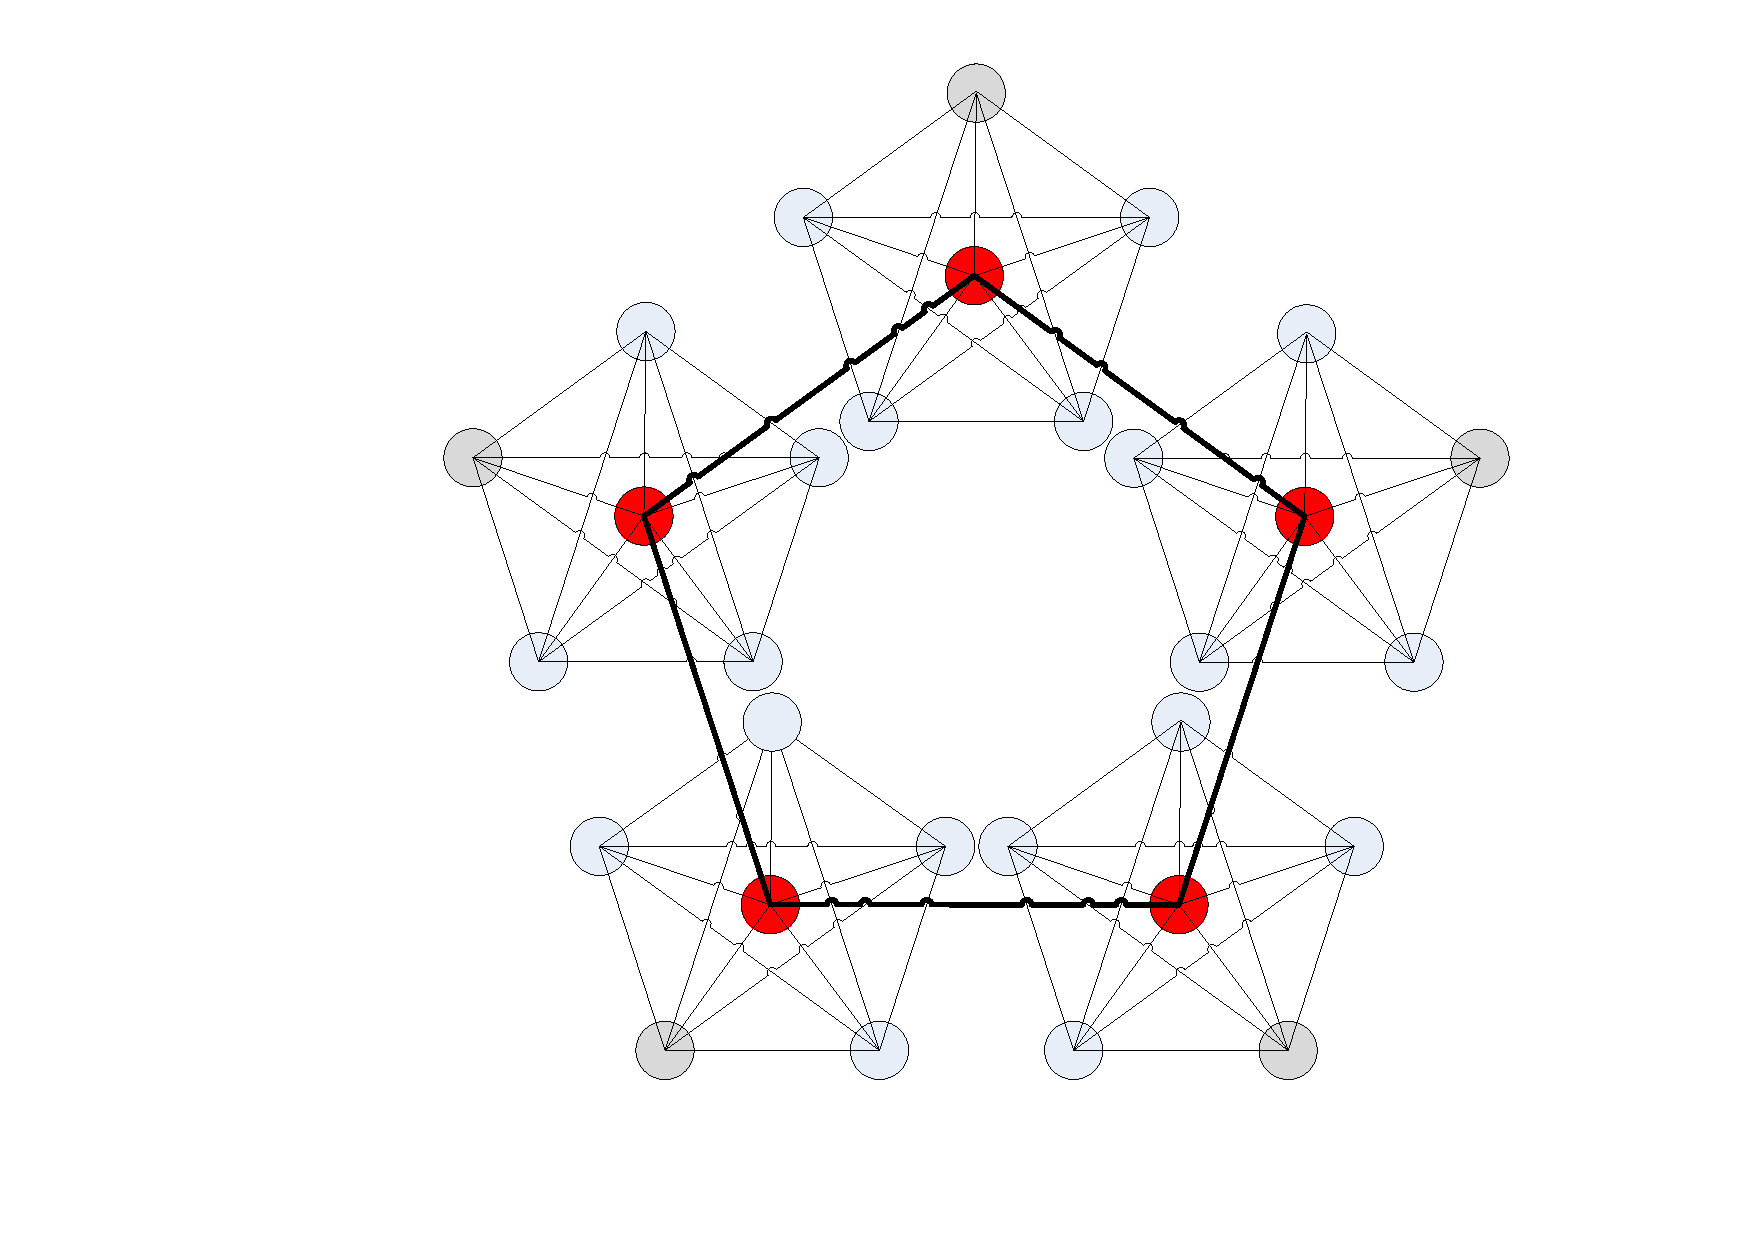
\includegraphics[clip=true, viewport=7.5cm 2.5cm 26cm 20cm, width=0.7\columnwidth]{CDHT_layout}
 \caption{Layout of the Pithos storage architecture}
 \label{fig_pithos}
\end{figure}
%
Figure \ref{fig_pithos} shows the structure of Pithos. The figure shows groups of fully connected peers (blue, grey and red), where all groups are
connected to each other in an P2P overlay through super peers (red). Backup peers are also present (grey), to take over responsibility if a super
peer leaves a group.

\subsection{Multi-tiered}

Pithos groups peers in some way, described in Section \ref{grouping}, to form a two tiered storage model. The first tier is a storage model at group
level and the second is a model over all groups. On the first tier, which is the intra group level, a fully distributed storage system is used to
allow for highly responsive read and write operations within the group. On the second tier, which is the inter group level, overlay routing is used
to store data between groups.

\subsection{Grouping}
\label{grouping}

At the core of the architecture will be how peers are grouped. One method by which peers might be grouped is merely to use peer proximity and
movement and thereby define groups as groups of users in the virtual world. The architecture will then make use of the flocking behaviour of players
to dynamically group players into flocks or clusters \cite{flocking}. The main idea of flocking is that players move around in groups, rather than
randomly on their own. Because of the flocking behaviour of players, dynamic groups or regions that move with groups of players may be a better fit
than static or even dynamic regions that operate on areas of the virtual world and not on how groups of players actually cluster.

If players are grouped more intelligently, less traffic will have to flow between groups, which will reduce the number of queries to the DHT, which
in turn will improve the latency of the overall system. Using groups or flocks would, therefore, compliment this technique.

The issue with such a system would be how to uniquely identify a group and how the identification would be applied when groups merge or split. Groups
moving towards each other also have to be identified and the grouping might have to be able to maintain two groups moving through each other.

Because a fully distributed architecture is not scalable, group sizes should also not exceed some threshold. This threshold complicates group
construction, because groups are already constructed according to position in the virtual world. Splitting groups might not be optimal, because the
supposition is that players close to each other require responsive access to each other's data as described in Section \ref{distance_based}. A
preferred solution might be to split groups into another tier using a grouped region approach. This will allow groups to remain scalable by allowing
for a inter group region communications method based on group-region super peers.

Little work has been done to group players in a distributed fashion in virtual worlds \cite{}. Further research is required into grouping algorithms
to determine their usability in virtual worlds under user churn.

As an alternative to geographic grouping, dynamic regioning might also be used to group players. Where every dynamic region will constitute a group
of players. Dynamic regioning splits an overpopulated region which will allow for sufficient bounding of the amount of players in the group.

\subsection{Distance-based}
\label{distance_based}

\subsection{Certification Authority}

Use secure node ID assignments, by making use of a Certification Authority, or designing the system in such a way that a peer cannot select or report
it's own node ID.

\subsection{Bootstrap mechanism}

\section{Implementation}
\label{implementation}

Pithos is being implemented in Oversim \cite{OverSim_2007}, running on Omnet++. Oversim was chosen because of the variety of already implemented
protocols as well as the layered architecture, which simplifies testing with different overlays and comparing with different storage types.

\subsection{Oversim architecture}

\begin{figure*}[htbp]
 \centering
 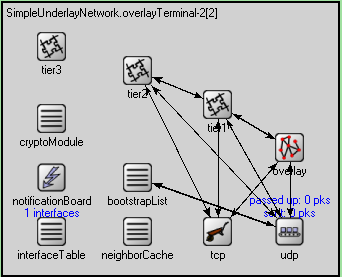
\includegraphics[width=\columnwidth]{Oversim_arch}
 \caption{Oversim architecture set up to use two tiers}
 \label{fig_oversim_arch}
\end{figure*}
%
Figure \ref{fig_oversim_arch} shows the layered Oversim architecture as displayed in Omnet++. The Oversim architecture consists of a network,
overlay, tier 1, tier 2 and tier 3 layers. The network layer implements TCP and UDP. Here it is possible to use a simple underlay network, where
nodes are positioned on Euclidean space and latencies are calculated according to the distances between nodes or to use a modified version of the
INET framework found in Omnet++, which attempts to accurately model latency effects and the various complexities of the underlying network.

The overlay layer contains the P2P overlay. Some overlays already implemented in Oversim include: Chord, Gia, Kademlia, Pastry, Quon and Vast.

The different tiers used in Oversim form the application layer of the OSI protocol stack, with tier 1 being the layer closest to the overly layer,
followed by tiers 2 and 3.

Pithos is developed as a tier 1 application, driven by a ``game'' module, which is implemented as a tier 2 application. The idea is that one can
empirically test different storage architectures by driving them with the same driver application and having them use the same overlay.

\subsection{Components}

Pithos consists of a few compound components that make up the architecture. Each compound component in turn consists of various simple components
that contain the Pithos code, written in C++.

\begin{figure*}[htbp]
\centering \subfloat[Peer)]{\label{fig_peer}
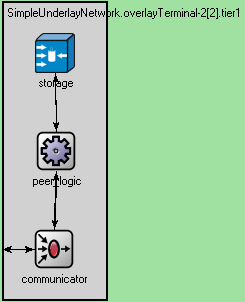
\includegraphics[width=0.815\columnwidth]{tier1_peer}}
 \subfloat[Super Peer]{\label{fig_super_peer}
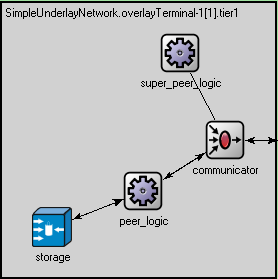
\includegraphics[width=\columnwidth]{tier1_super_peer}}
\caption{Tier 1 modules}
\end{figure*}

The compound component types contained in Pithos are Super Peers, Peers and the Directory Server. The directory server only consists out of the
Directory Logic simple module. Figure \ref{fig_peer} shows the Peer compound module, consisting of Peer Logic, Storage and Communicator simple
modules. Figure \ref{fig_super_peer} shows the Super Peer compound module, consisting of Super Peer Logic, Peer Logic, Storage and Communicator
simple modules. The same modules are present in both Super Peers and Peers, because Super Peers are seen as Peers with extra intelligence. Any Peer
can theoretically become a Super Peer by just creating a Super Peer Logic module for itself.

When a Super Peer is created, it registers its IP address and position within the virtual world with the Directory Server. When a peer joins the
network it sends its position to the directory server and receives a super peer IP that is closest in return. A joining peer then sends a request to
join a group

\subsection{Network setup}

\subsection{Future work}

%Use KBRTestApp

\section{Preliminary results}
\label{results}

\section{Conclusion}
\label{conclusion}

\subsection{Summary}

\subsection{Future work}


%\newpage
% use section* for acknowledgement
\ifCLASSOPTIONcompsoc
  % The Computer Society usually uses the plural form
  \section*{Acknowledgments}
\else
  % regular IEEE prefers the singular form
  \section*{Acknowledgment}
\fi

The financial assistance of MIH and the National Research Foundation (NRF) towards this research is hereby acknowledged. Opinions expressed and
conclusions arrived at, are those of the author and are not necessarily to be attributed to MIH or the NRF.

%\newpage
%\IEEEtriggeratref{43} %Balance the bibliography
\bibliographystyle{IEEEtran}
\bibliography{../BibTeX/P2P_MMOG}

% that's all folks
\end{document}
